%%%%%%%%%%%%%%%%%%%%%%%%%%%%%%%%%%%%
%%%%%%%%%% USER INTERFACE %%%%%%%%%%
%%%%%%%%%%%%%%%%%%%%%%%%%%%%%%%%%%%%
\section{User interface}
\writer{Jerome}
This chapter describes the main aspects regarding how the User Interface of our Software product looks.

%%%%%%%%%% TECHNOLOGIES %%%%%%%%%%
\subsection{Technologies}
The GUI shall be implemented using Eclipse plugins. These plugins are of various types and together work to obtain the desired functionality. The used types are:

\begin{description}
  \item[Editor] - used for the creation and edition of the different resources (Resource Editor) to design the networks according to the desired specifications.
  \item[View] - show the different properties of the resource currently being edited (Diagram Overview).
  \item[Pop-up] - used to add extra functionalities (Right-click Menu).
\end{description}

%%%%%%%%%% GUI PARTS %%%%%%%%%%
\subsection{GUI parts}
In this section, we will talk in more details about all the different parts of the global editor running in Eclipse that will be provided with the software. Throughout this document we will refer to this as the Workbench. The Workbench is composed of five main parts as shown in Figure \ref{fig:gui_editors}: the Project Explorer, the Resource Editor, the Properties View, the Diagram Overview and finally the ToolBar.

The most important components are the Project Explorer, the Resource Editor and the Properties View because they allow the user to interact with the software, creating new parts or editing them. In the following sections a short description of all the different parts will be provided.

\begin{figure}[htp]
\begin{center}
  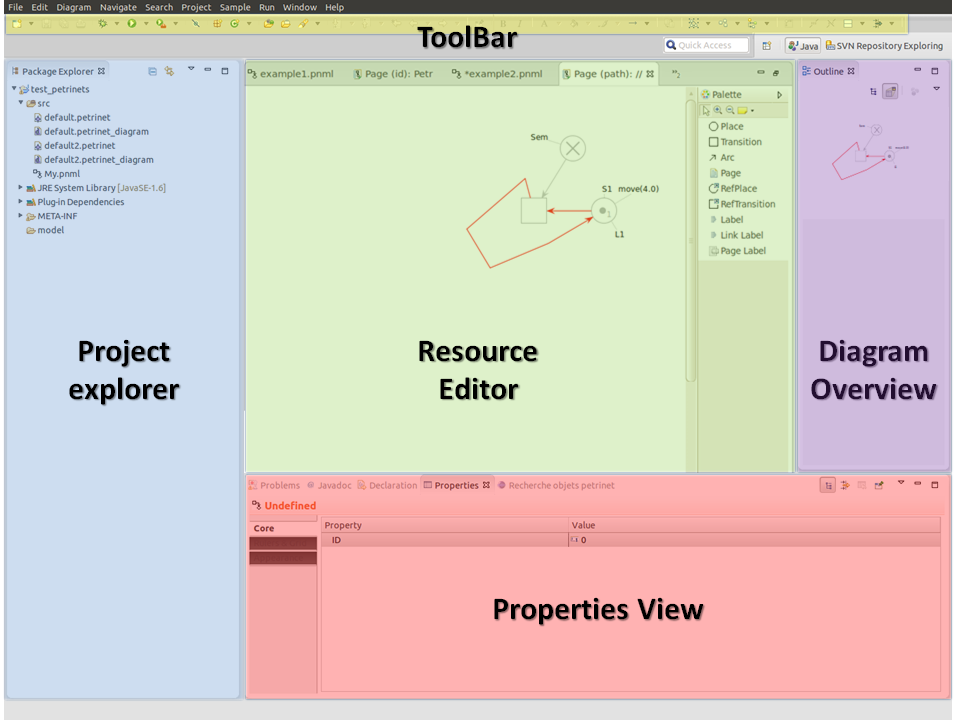
\includegraphics[scale=0.45]{image/gui_editors.png}
  \caption{Workbench}
  \label{fig:gui_editors}
\end{center}
\end{figure}

%%%%% Project Explorer %%%%%
\subsubsection{Project Explorer}
The Project Explorer is a standard Eclipse view. It provides the user with an overview of the project showing the different folders and files composing it, with their extensions. By selecting a file and pressing Enter, the view will determine what type of file the user has selected and open the Editor associated with this type of file (see Figure \ref{fig:gui_file_editor}).

\begin{figure}[htp]
\begin{center}
  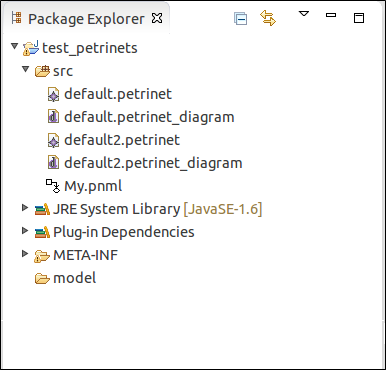
\includegraphics[scale=0.45]{image/gui_file_editor.png}
  \caption{Eclipse Project Explorer}
  \label{fig:gui_file_editor}
\end{center}
\end{figure}

%%%%% Resource Editor %%%%%
\subsubsection{Resource Editor}
This part of the Workbench is an Editor, more precisely a set of Editors. In the following figure you will see a representation of the Petri net Editor,
which allows the user to create, design and modify Petri nets. (See Figure \ref{fig:gui_petri_editor}).

\begin{figure}[htp]
\begin{center}
  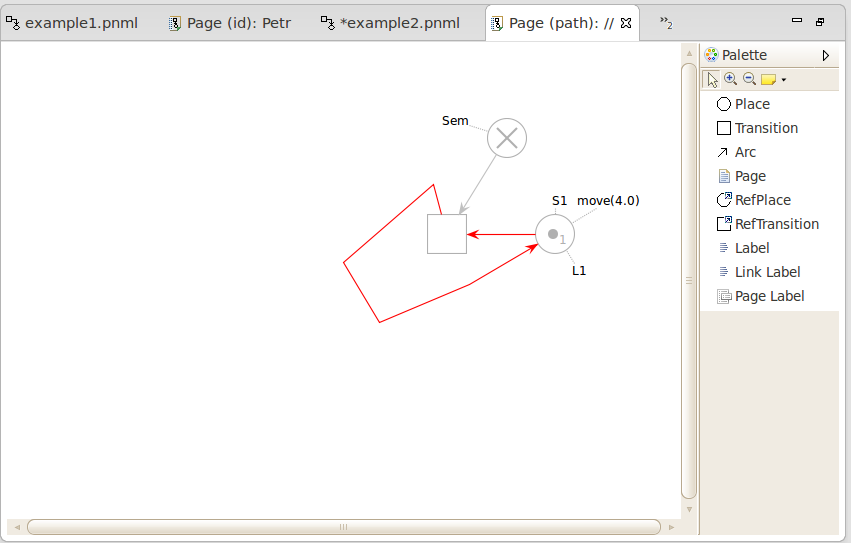
\includegraphics[scale=0.45]{image/gui_petrinet.png}
  \caption{Petri net Editor}
  \label{fig:gui_petri_editor}
\end{center}
\end{figure}

The Resource Editor is split into two parts : the left area contains a graphical representation of the resource the user is editing while the right area displays a
Palette of elements that the user can drag and drop to modify the graphical part.

In the graphical representation, the user is allowed to move elements, resize them and edit their name by double-clicking on them. The Palette contains some other useful tools such as zooming and adding notes in the graphical representation so the user can explain to another user some parts of his representation. In addition to the Petri net Editor, we also have three other Editors provided with our software: the Geometry Editor that allows the user to draw a shape (for example, the shape of the track) that will be associated with the Petri net for the simulation (See Figure \ref{fig:gui_geometry_editor}); the Appearance Editor that provides a way to edit the appearance of Places and Tokens; and the Configuration Editor that keeps a reference to the Petri net Model and the Geometry Model to configure the simulation.

\begin{figure}[htp]
\begin{center}
  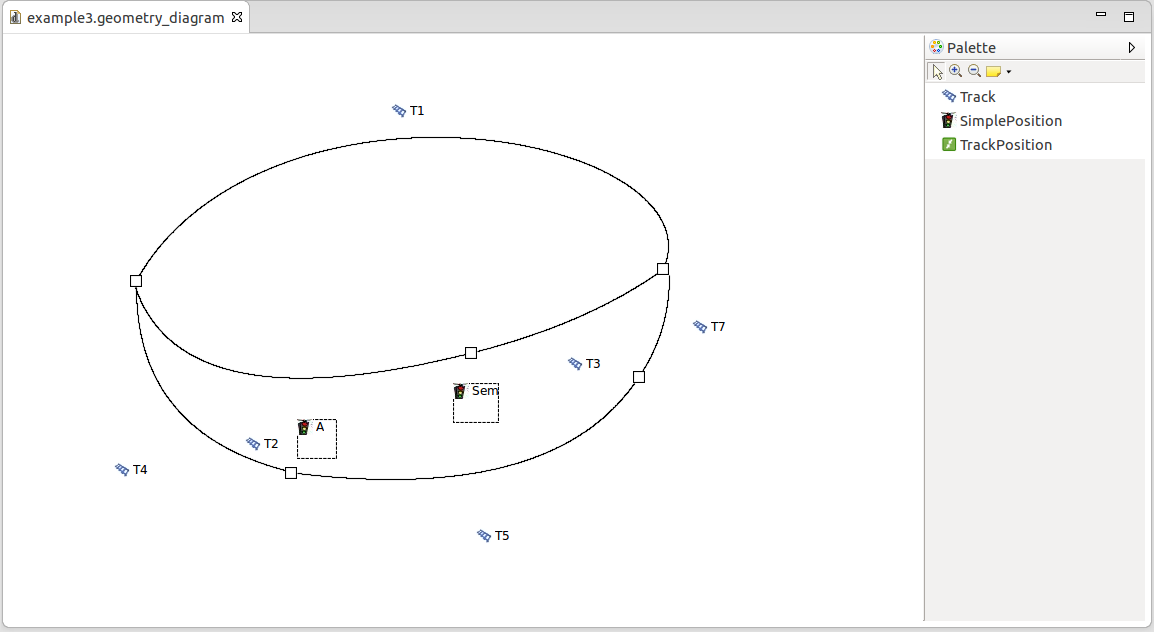
\includegraphics[scale=0.45]{image/gui_geometry_editor.png}
  \caption{Geometry Editor}
  \label{fig:gui_geometry_editor}
\end{center}
\end{figure}

%%%%% Properties View %%%%%
\subsubsection{Properties View}
The Properties View is another one Eclipse built-in plugin displayed as a view. This view is connected to the Resource Editor and displays some additional properties depending on the selected object. The goal of the Properties View is to edit the properties of different objects of the diagram. The Figure \ref{fig:gui_property_editor} below will for example provide you the Properties View associated with the selection of a Transition in our Petri net editor.

\begin{figure}[htp]
\begin{center}
  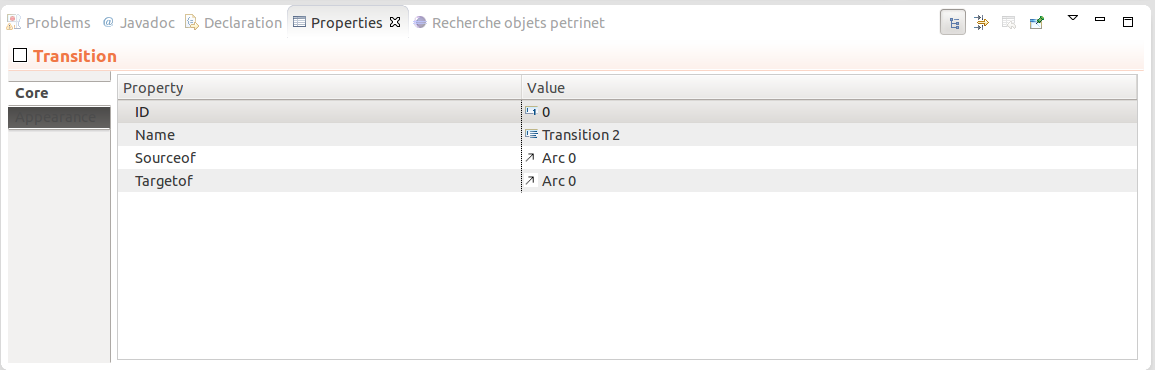
\includegraphics[scale=0.30]{image/gui_property_editor.png}
  \caption{Property View}
  \label{fig:gui_property_editor}
\end{center}
\end{figure}

%%%%% Diagram Overview %%%%%
\subsubsection{Diagram Overview}
One more useful Eclipse plugin is the Diagram Overview, also implemented as a view. The particularity of this view is that its goal is to show a global view of the Diagram we are editing with a box symbolizing the part we are actually seeing in the Resource Editor. As a diagram can be a lot bigger than the user's screen this plugin is used to navigate through the Diagram as the Resource Editor will display what is inside the box and we can move the ``seeing box'' dragging it in the Diagram Overview (see Figure \ref{fig:gui_diagram_overview}).

\begin{figure}[htp]
\begin{center}
  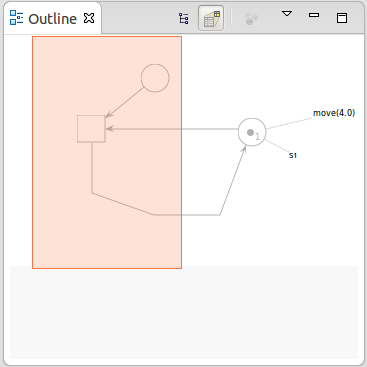
\includegraphics[scale=0.50]{image/gui_diagram_overview.png}
  \caption{Seeing box}
  \label{fig:gui_diagram_overview}
\end{center}
\end{figure}

%%%%% Tool Bar %%%%%
\subsubsection{ToolBar}
The ToolBar is the area in Eclipse where all the general functions are placed. This includes commands like creating, saving and loading, next and previous page, etc (see Figure \ref{fig:gui_toolbar}).

\begin{figure}[htp]
\begin{center}
  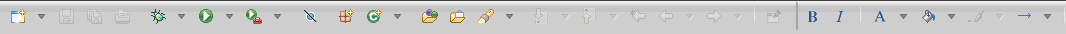
\includegraphics[scale=0.40]{image/gui_toolbar.png}
  \caption{Toolbar}
  \label{fig:gui_toolbar}
\end{center}
\end{figure}

%%%%% Right Click Meny %%%%%
\subsubsection{Right-click Menu}
This global menu (in the sense it can be accessed everywhere) is not shown in our Figure \ref{fig:gui_editors}. It can be triggered by the user pressing the right button of his mouse. It will show some relevant options such as delete object, or start some actions. Indeed each content of the menu will depend of the type of selected component. As an example, we can show the "Start Simulation" action that has been implemented in \epns. This function is only available when a right-click is performed on a ``Configurator'' object and allows launching of the Simulation and the Visualization for the Petri net  (see Figure \ref{fig:gui_popup_menu}).

\begin{figure}[htp]
\begin{center}
  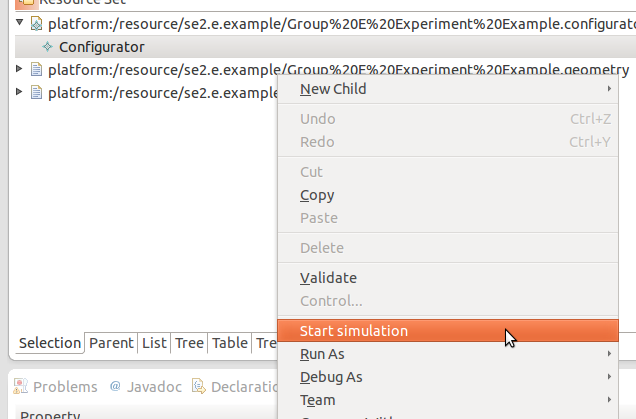
\includegraphics[scale=0.40]{image/gui_popup_menu.png}
  \caption{Right-click Menu}
  \label{fig:gui_popup_menu}
\end{center}
\end{figure}

%%%%% Simulator %%%%%
\subsubsection{Simulator and Graphical Visualization}
\index{Simulator!UI}
This last component is also not shown in Figure~\ref{fig:gui_editors} as it is a window detached
from Eclipse. It provides a 3D visualisation of a chosen Petri net using the Geometry Model and the
Appearance Model that have been set up earlier. It has two main buttons: Start/Stop and Pause/Resume
allowing the user to control the simulation \& visualization. The user may also interact with the
tool by clicking on the interactive input places in the simulator to trigger events, for example to
change the status of a a traffic light from the red to the green state (see Figure
\ref{fig:gui_simulator}).

\begin{figure}[htp]
\begin{center}
  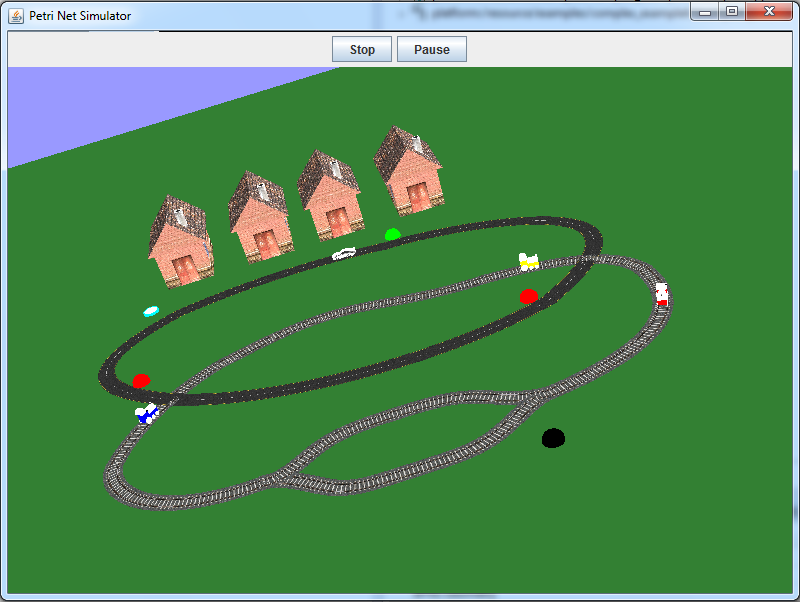
\includegraphics[scale=0.50]{image/gui_simulator.png}
  \caption{The Simulator}
  \label{fig:gui_simulator}
\end{center}
\end{figure}
